\documentclass{article}
\usepackage[T1]{fontenc}
\usepackage{lmodern}
\usepackage{graphicx}
\usepackage{amsmath,amssymb}
\usepackage[a4paper,margin=2cm]{geometry}
\usepackage[absolute,overlay]{textpos}
\setlength{\TPHorizModule}{1mm}
\setlength{\TPVertModule}{1mm}
\usepackage[indonesian]{babel}
\usepackage{hyperref}
\setlength{\emergencystretch}{2em}
% unit: Halaman 78

\begin{document}

% === Halaman 78 (llm) ===

Plainteks: temui ibu nanti malam

Bigram: te mu ix ib un an ti ma la mx

\vspace{10mm}

Kunci: 

\vspace{10mm}

Cipherteks: ZB RS FY KU PG LG RK VS NL QV

% deskripsi: Tabel kunci kriptografi berupa grid 5x5 yang berisi huruf-huruf alfabet (tanpa huruf J) untuk proses enkripsi.
% bbox normalisasi: [0.1970, 0.2770, 0.4200, 0.6400]
\begin{textblock*}{46.83mm}(41.37mm,82.27mm)
\noindent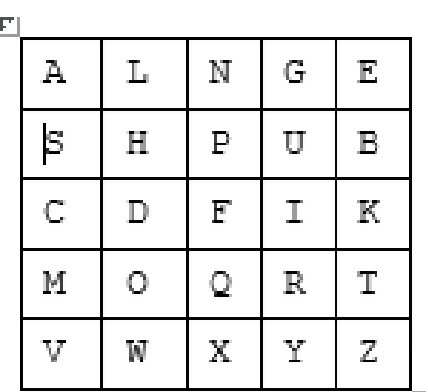
\includegraphics[width=46.83mm,height=107.81mm]{../../images/llm/page_078_img_01.png}%
\end{textblock*}

\end{document}
